\documentclass{article}
\usepackage[paperwidth=17cm,paperheight=7.5cm,margin=0.25cm]{geometry}
\usepackage[T1]{fontenc}\usepackage{lmodern,tikz,xcolor}
\usetikzlibrary{positioning,calc}
\pagestyle{empty}\setlength{\parindent}{0pt}
\definecolor{navy}{HTML}{17365D}
\definecolor{power}{HTML}{B92727}
\definecolor{sda}{HTML}{16815D}
\definecolor{scl}{HTML}{165FAA}
\tikzset{every node/.style={font=\small},box/.style={draw=navy,rounded corners,fill=blue!3},wire/.style={line width=1.1pt}}
\begin{document}\centering
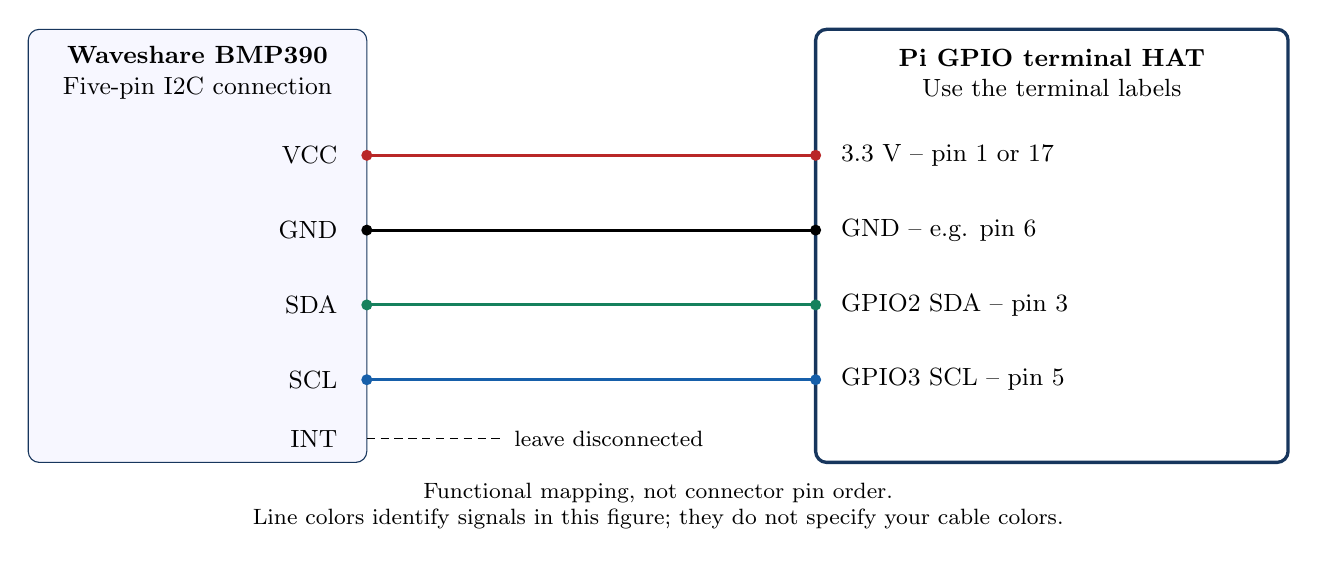
\begin{tikzpicture}[x=1cm,y=1cm]
\draw[box] (0,0) rectangle (4.3,5.5);
\node[align=center] at (2.15,4.95){\textbf{Waveshare BMP390}\\Five-pin I2C connection};
\draw[draw=navy,very thick,fill=white,rounded corners] (10,0) rectangle (16,5.5);
\node[align=center] at (13,4.95){\textbf{Pi GPIO terminal HAT}\\Use the terminal labels};
\foreach \y/\a/\b/\c in {3.9/VCC/3.3 V -- pin 1 or 17/power,2.95/GND/GND -- e.g. pin 6/black,2.0/SDA/GPIO2 SDA -- pin 3/sda,1.05/SCL/GPIO3 SCL -- pin 5/scl}{
 \node[anchor=east] at (4.05,\y){\a};
 \node[anchor=west] at (10.2,\y){\b};
 \draw[wire,\c] (4.3,\y)--(10,\y);
 \fill[\c] (4.3,\y) circle(2pt);\fill[\c] (10,\y) circle(2pt);
}
\node[anchor=east] at (4.05,0.3){INT};
\draw[densely dashed] (4.3,0.3)--(6.0,0.3);
\node[anchor=west,font=\footnotesize] at (6.05,0.3){leave disconnected};
\node[align=center,font=\footnotesize] at (8,-0.55){Functional mapping, not connector pin order.\\Line colors identify signals in this figure; they do not specify your cable colors.};
\end{tikzpicture}
\end{document}
